 % \documentclass[sigconf]{acmart}
\documentclass{article}
% We want page numbers on submissions

%%\ccsPaper{9999} % TODO: replace with your paper number once obtained

%packages
\usepackage{natbib}
\usepackage{amsmath}
\usepackage{amsthm}
\usepackage{mathtools}
\usepackage{mdframed}
\usepackage{subfigure}
\usepackage{booktabs}
% \usepackage{hyperref}
\usepackage{subfigure}
\usepackage{siunitx} % Provides the \SI{}{} and \si{} command for typesetting SI units
\usepackage{graphicx} % Required for the inclusion of images
% \usepackage{natbib} % Required to change bibliography style to APA
\usepackage{datetime}
\usepackage{lscape}
\usepackage{algorithm}
\usepackage{algorithmic}
\usepackage{xspace}
\usepackage[english]{babel} % English language/hyphenation
\usepackage{proof}
\usepackage{booktabs} % Top and bottom rules for tables
\usepackage[colorlinks, allcolors = blue,]{hyperref}
\usepackage{accents}
\usepackage{amsfonts}
\usepackage{stmaryrd}
\usepackage{amsmath,amsthm,amssymb,latexsym} 
\usepackage{microtype}
\usepackage{graphicx}
\usepackage{subfigure}
\usepackage{booktabs} % for professional tables
\usepackage{hyperref}
\usepackage{icml2019}
\usepackage{lipsum}

\usepackage{authblk}


%new commands
\newcommand{\theHalgorithm}{\arabic{algorithm}}
\newtheorem{definition}{Definition}
\usepackage{cancel}
\usepackage[normalem]{ulem}
\newcommand{\dataobs}{\textbf{x}}
\newcommand{\adj}[2]{\textbf{adj}(#1,#2)}
\newcommand{\candidateset}{\mathcal{R}_{\textup{post}}}
\newcommand{\bprior}{\boldsymbol{\beta}_{\textup{prior}}}
\newcommand{\bysinfer}{\mathsf{Infer}}
\newcommand{\betad}{\mathsf{Beta}}
\newcommand{\betaf}{\textup{B}}
\newcommand{\mbetaf}{\boldsymbol{\textup{B}}}
\newcommand{\vtheta}{\boldsymbol{\theta}}
\newcommand{\valpha}{\boldsymbol{\alpha}}
\newcommand{\vbeta}{\boldsymbol{\beta}}
\newcommand{\lapmech}{\mathsf{LSDim}}
\newcommand{\ilapmech}{\mathsf{LSHist}}
\newcommand{\binomial}[2]{\mathsf{Bin}(#1, #2)}
\newcommand{\multinomial}[2]{\mathsf{Mult}(#1, #2)}
\newcommand{\expmech}{\mathsf{EHD}}
\newcommand{\hexpmech}{\mathsf{EHDS}}
\newcommand{\lexpmech}{\mathsf{EHDL}}
\newcommand{\hexpmechd}{\mathsf{expMech}^{D}_{\hellinger}}
\newcommand{\privinfer}{\mathsf{PrivInfer}}
\newcommand{\hlg}{\mathsf{H}}
\newcommand{\dirichlet}[1]{\mathsf{Dir}(#1)}
\newcommand{\alphas}{\boldsymbol{\alpha}}
\newcommand{\xis}{\boldsymbol{\xi}}
\newcommand{\iverson}[1]{[#1]}
\newcommand{\datauni}{\mathcal{X}}
\newcommand{\hellinger}{\mathcal{H}}
\newcommand{\ux}[1]{u(\textbf{x}, {#1})}
\newcommand{\uxadj}[1]{u(\textbf{x}', {#1})}
\newcommand{\cardinality}[2]{\mathcal{C}^{#1}_{#2}}
\newcommand{\range}{\mathcal{O}}
\newcommand{\nomalizer}[1]{\sum\limits_{r'\in \mathcal{R}_{\textup{post}}} \exp \big(\frac{-\epsilon\cdot \mathcal{H} (\mathsf{BI}(#1),r')}{4 \cdot S(#1)}\big)}

\newcommand{\unomalizer}[1]{\sum\limits_{r'\in \mathcal{R}_{\textup{post}}} \exp \big(\frac{-\epsilon\cdot u(#1, r')}{4 \cdot S(#1)}\big)}


\newcommand{\hexpmechPr}[2]{\underset{z \thicksim \hexpmech(#1)}{\Pr}\left[ #2 \right]}
\newcommand{\lapmechPr}[2]{\underset{z \thicksim \lapmech(#1)}{\Pr}\left[ #2 \right]}

\newcommand{\ilapmechPr}[2]{\underset{
{z \thicksim \ilapmech(#1)}
}{\Pr}\left[ #2 \right]}

\newtheorem{thm}{Theorem}[section]

\newtheorem{lem}{Lemma}[section]

\newtheorem{assert}{Assertion}[lem]
\newcommand{\lap}[2]{\mathsf{Lap}(#1, #2)}
\newcommand{\todo}[1]{{\footnotesize \color{red}\textbf{[[ #1 ]]}}}
\icmltitlerunning{Exploring the Design Space of Differentially Private
  Bayesian Inference under Hellinger Distance}

\begin{document}

\twocolumn[
\icmltitle{Exploring the Design Space of Differentially Private
  Bayesian Inference under Hellinger Distance}

% It is OKAY to include author information, even for blind
% submissions: the style file will automatically remove it for you
% unless you've provided the [accepted] option to the icml2019
% package.

% List of affiliations: The first argument should be a (short)
% identifier you will use later to specify author affiliations
% Academic affiliations should list Department, University, City, Region, Country
% Industry affiliations should list Company, City, Region, Country

% You can specify symbols, otherwise they are numbered in order.
% Ideally, you should not use this facility. Affiliations will be numbered
% in order of appearance and this is the preferred way.
\icmlsetsymbol{equal}{*}

\begin{icmlauthorlist}
\icmlauthor{Jiawen Liu}{to}
\icmlauthor{Gian Pietro Farina}{to}
\icmlauthor{Tetsuya Sato}{to}
\icmlauthor{Mark Bun}{ed}
\icmlauthor{Marco Gaboardi}{to}
\end{icmlauthorlist}

\icmlaffiliation{to}{Department of Computer Science and Engineering, University at Buffalo, SUNY, New York, United States}
\icmlaffiliation{ed}{Princeton University, United States}

% \icmlcorrespondingauthor{Cieua Vvvvv}{c.vvvvv@googol.com}
% \icmlcorrespondingauthor{Eee Pppp}{ep@eden.co.uk}

% You may provide any keywords that you
% find helpful for describing your paper; these are used to populate
% the "keywords" metadata in the PDF but will not be shown in the document
\icmlkeywords{Machine Learning, ICML}

\vskip 0.3in
]

\printAffiliationsAndNotice{\icmlEqualContribution} % otherwise use the standard text.

\begin{abstract}
% Several approaches have been explored in order to make Bayesian inference
% differentially private.
% For instance, \cite{dimitrakakis2014robust} and
% \cite{wang2015privacy} proved that, under specific conditions of the likelihood function and the prior distribution,
% sampling from the posterior distribution, is already differentially private. \cite{zhang2016differential} and \cite{foulds2016theory}
% designed differentially private (d.p.) mechanisms by adding laplacian noise
% to the numeric parameters of the posterior distributions. 
% Accuracy, is usally (\cite{??}) measured by providing upper bounds, holding w.h.p, on the
% $\ell_1$ or $\ell_\infty$-distance between the numeric parameters
% of the released posterior distribution and the actual real ones of posterior distribution.
We explore the design space of differentially private Bayesian
inference mechanisms with accuracy measured in terms of Hellinger
distance over posterior distributions.  
We focus on two discrete models for parametric Bayesian
inference: the Beta-Binomial and the Dirichlet-Multinomial
models. We study two mechanisms based on the 
Laplace perturbation of the parameters of the posterior distribution under
$\ell_1$ norm, and compare them with a discrete mechanism calibrating 
its score function to a smooth bound on the Hellinger distance.
Accuracy is measured through the Hellinger distance between the posterior
distribution released by the different mechanisms and the real one.
We compare the accuracy theoretically and experimentally.
\end{abstract}
 % TODO: replace with your keywords





\section{Introduction}
\label{sec_intro}
Data analysis techniques have brought significant improvements in a
variety of applications including applications from the medical,
financial, social, and transportation fields. In order to provide
better services, these applications need large amounts of users data
putting at risk the privacy of individual users contributing their data. 
Differential privacy was proposed a decade ago to address these
situations and it on its way to become a gold standard in data
privacy.  

Bayesian inference is a standard statistical tool that is useful to
estimate a posterior distribution when given a prior distribution and
some observed data. 

In this work we consider the design space of  parametric Bayesian
inference mechanisms guaranteeing differential privacy. Our work is
motivated by recent developments in the area of probabilistic
programming where several tools have been proposed to perfor
parametric and non-parametric Bayesian inference in an efficient
way. The in
for our work is the recent development of 

In particular
we focus on two classical models: the Beta-Binomial and the
Dirichlet-Multinomial models. These are classical models 


Our work is conducted under a Bayesian inference scenario, where the posterior distribution is the analysis result we obtained from the data.
Publishing the posterior distribution inferred from a sensitive dataset can
leak information about the individuals in the dataset.
In order to guarantee differential privacy and to protect the
individuals' data we can add noise to the posterior before releasing it.
The amount of the noise that we need to introduced
depends on the privacy parameter $\epsilon$ and the sensitivity of the inference to
small changes in the data set. 
Sensitivity can be computed in many different ways based on which metric space
we consider on the output set of the mechanism. In the literature on private Bayesian
inference (\cite{zhang2016differential,xiao2012bayesian}), it is only measured with
respect to the vector of numbers parametrizing the output distribution using, e.g. the $\ell_1$ norm.
A more natural approach which we explore here, is to measure sensitivity with respect to a metric on the space of inferred probability distributions.
A re-loved question is that of how to measure accuracy. Again,
this can be answered in different ways based on the metric imposed on the output space, and yet again
only in few works in literature (e.g. \cite{zhang2016differential})
distances between probability measures have been used for these purposes.


The question that this work aims at answering is whether
an approach based on probability metrics can improve on
the accuracy of approaches based on metrics over
the numeric parameters of the distributions. 
We will see that in some cases this can happen.

\noindent \textbf{Main contributions.}
\begin{itemize}
	\item We design a new differentially private Bayesian inference mechanism based on the standard exponential mechanism.

	\item We explored two ways to improve the accuracy: 1) calibrating noise to the sensitivity of a metric over distributions (e.g. Hellinger distance ($\hellinger$), $f$-divergences, etc\dots). 2) Using a smooth upper bound on the local sensitivity and scale the noise to this smooth bound rather than global sensitivity, to improve the mechanism accuracy.

  \item A full proof on the newly designed mechanism is $(\epsilon, \delta)-$differential privacy is given in paper.

	\item We implemented the new proposed mechanism and other art-of-state mechanisms, comparing the performance in terms of accuracy and privacy.
\end{itemize}


\section{Preliminaries}
\label{sec_background}
\noindent \textbf{Bayesian inference.} 
Given a prior belief $\Pr(\theta)$ on some parameter $\theta$,
and an observation $\dataobs$, the posterior distribution on $\theta$ given $\dataobs$ is defined as:
\[
  \Pr(\theta | \dataobs) \equiv \frac{\Pr(\dataobs | \theta) \cdot \Pr(\theta)}{\Pr(\dataobs)}
\]
where the expression $\Pr(\dataobs | \theta)$ denotes the
\emph{likelihood} of observing $\dataobs$ under a value of
$\theta$. Since we consider $\dataobs$ to be fixed, the likelihood is
a function of $\theta$.
For the same reason $\Pr(\dataobs)$ is a constant independent of $\theta$.
Usually in statistics the prior distribution $\Pr(\theta)$ is chosen so that it represents
the initial belief on $\theta$, that is, when no data has been observed. In practice though,
prior distributions and likelihood functions are usually chosen so that the posterior
belongs to the same \emph{family} of distribution of the prior. In this case we say that the prior
is conjugate to the likelihood function. Use of a conjugate prior
simplifies calculations and allows for inference to be performed in a
recursive fashion over the data.
% Then, we have:
% \[
%   \bysinfer(\Pr(\dataobs | \theta), \Pr(\theta), \dataobs) = \frac{\Pr(\dataobs | \theta) \cdot \Pr(\theta)}{\Pr(\dataobs)}
% \]
% \noindent \textbf{Beta-binomial System.}
In this work we will consider a specific instance of Bayesian inference and one of its generalizations.
We will consider the situation where the underlying data is drawn from a binomial distribution
($\thicksim \binomial{n}{\theta}$), where $\theta$ represents
the parameter --informally called \emph{bias}-- of a Bernoulli
distributed random variable and $n$ is the number of draws. The
prior distribution over $\theta\in [0,1]$ is going to be a beta
distribution, $\betad(\alpha, \beta)$, with parameters
$\alpha,\beta\in\mathbb{R}^{+}$, and with p.d.f:
\[
  \Pr(\theta)\equiv \frac{\theta^{\alpha} (1- \theta)^{\beta}}{\betaf(\alpha,\beta)}
\]
where $\betaf(\cdot,\cdot)$ is the beta function.
The data $\dataobs$ will be a sequence of $n\in\mathbb{N}$ binary values, that is $\dataobs= (x_1,\dots x_n), x_i\in\{0,1\}$, and the likelihood function is:
\[
  \Pr(\dataobs | \theta)\equiv \theta^{\Delta \alpha}(1-\theta)^{n - \Delta \alpha}
\]
where $\Delta \alpha = \displaystyle\sum_{i=1}^{n}x_i$.
The posterior distribution over $\theta$ can be easily proven to be equal to:\[\betad(\alpha + \Delta \alpha,\beta + n - \Delta \alpha)\]
From now on we will denote by $\bysinfer(\binomial{n}{\theta}, \betad(\alpha, \beta), \dataobs)$ the previous
posterior distribution. This notation will prove itself handy when its arguments will change types in the next example and
in section \ref{} when the private mechanisms will be described.
% \noindent \textbf{Dirichlet-multinomial Systems.}


The beta-binomial model can be immediately generalized to the Dirichlet-multinomial model, with underlying data multinomially distributed.
The \emph{bias} is represented by the parameter $\vtheta$, the vector of parameters of a categorically distributed random variable. The prior distribution over $\vtheta\in [0,1]^{k}$
is given by a Dirichlet distribution, $\dirichlet{\valpha}$, for $k\in\mathbb{N}$,
and $\valpha\in(\mathbb{R}^{+})^{k}$, with p.d.f:
\[
  \Pr(\vtheta)\equiv\frac{1}{\mbetaf(\valpha)}\cdot \displaystyle\prod_{i=1}^{k}{\theta_i^{\alpha_i-1}}
\]
where $\mbetaf(\cdot)$ is the generalized beta function.
The data $\dataobs$ will be a sequence of $n\in\mathbb{N}$ values
coming from a universe $\datauni$, such that $\mid\datauni \mid=k$.
The likelihood function will be:
\[
  \Pr(\dataobs|\vtheta)\equiv \displaystyle\prod_{a_i\in\datauni}\theta_{i}^{\Delta \alpha_i},
\]
with $\Delta \alpha_i=\displaystyle\sum_{j=1}^{n}\iverson{x_j=a_i}$, where $\iverson{\cdot}$ represents Iverson bracket notation.
Denoting by $\Delta\valpha$ the vector $(\Delta\alpha_1,\dots \Delta\alpha_k)$ the posterior distribution over $\vtheta$ turns out to be
\[
   \bysinfer(\multinomial{n}{\vtheta}, \dirichlet{\valpha}, \dataobs)=\dirichlet{\valpha + \Delta \valpha} 
\]
where $+$ denotes the componentwise sum of vectors of reals.


\noindent \textbf{Differential Privacy.}
\emph{Differential privacy} is a strong quantitative notion of statistical privacy proposed by \cite{}.
Differential privacy of a mechanism implies that changing the input of a mechanism slightly only reflects
in a controlled and bounded way on the output distribution. 
Formally, the $\epsilon$ parameter
controls how much two outputs starting from \emph{close} inputs can differ. When two inputs are close we call them \emph{adjacent}.
By adjacency we usually mean a relation over input databases which includes all the pair of databases which differ by at most one row.
The formal definition of $\epsilon$-differential privacy follows.
\begin{definition}
\label{def_epsilon_dp}

A randomized mechanism $\mathcal{M}$ with domain $\mathbb{N}^{|\mathcal{X}|}$ and codomain $\range$, is $\epsilon$-differential private, if for all adjacent
\footnote{Given $\dataobs, \dataobs'\in\{0,1\}^n$  we say that $\dataobs$ and $\dataobs'$ are adjacent and we write, iff
$\displaystyle \sum_{i}^{n}\iverson{x_i = x'_i }\leq 1$. } $\dataobs, \dataobs' \in \mathbb{N}^{|\mathcal{X}|}$ and all $\mathcal{S} \subseteq \range$:
\begin{equation*}
\Pr[\mathcal{M}(\dataobs) \in \mathcal{S}] \leq e^\epsilon \Pr[\mathcal{M}(\dataobs') \in \mathcal{S}].
\end{equation*}

\end{definition}


\noindent \textbf{Technical Problem Statement.}
\label{subsec_problem}
We are interested in exploring mechanisms for privately releasing the full posterior
distributions derived in section \ref{sec_background}, as opposed to just sampling from them.
It's worth noticing that the posterior distributions are fully characterized
by their parameters, and the family (Beta, Dirichlet distribution) they belong to. Hence, in case of the
Beta-Binomial model we are interested in releasing a private version of the pair of
parameters $(\alpha',\beta')=(\alpha + \Delta \alpha,\beta + n - \Delta \alpha)$, and
in the case of the Dirichlet-multinomial model we are interested in a private version of
$\valpha'=(\valpha + \Delta \valpha)$. \cite{zhang2016differential} and \cite{xiao2012bayesian}
have already attacked this problem by adding independent Laplacian noise to the
parameters of the posteriors. That is, in the case of the Beta-Binomial system,
the value released would be: $(\tilde\alpha,\tilde\beta)=(\alpha +  \widetilde{\Delta \alpha},\beta + n - \widetilde{\Delta \alpha})$
where $\widetilde{\Delta \alpha}\thicksim \lap{\Delta \alpha}{\frac{2}{\epsilon}}$,
and where $\lap{\mu}{\nu}$ denotes a Laplace random variable with mean $\mu$ and scale $\nu$.
This mechanism is $\epsilon$-differentially private, and the noise is
calibrated w.r.t. to a sensitivity of 2 which is derived by using
$\ell_1$ norm over the pair of parameters. Indeed, considering two
adjacent data observations $\dataobs, \dataobs'$, that, from a unique prior, give rise to two posterior
distributions, characterized by the pairs
$(\alpha',\beta')$ and $(\alpha'',\beta'')$ then
$|\alpha'-\alpha''|+|\beta'-\beta''|\leq 2$.
This argument extends similarly to the Dirichelet-Multinomial system. Details are introduced in Sec. \ref{sec_mechs}.\\
However, in previous works, the accuracy of the posterior was measured with respect to $\ell_1$ norm. That is, an upper bound was given on
\[
  \Pr[|\alpha - \tilde\alpha| + |\beta - \tilde\beta |\geq \gamma ]
\]
where $(\alpha, \beta), (\tilde\alpha,\tilde\beta)$ are as defined above.
\todo{However, distance between
distributions are more naturally to be measured by distribution
metrics such as $f$-divergence, Hellinger distance, etc., than the $\ell_1$ norm shown above.}
{\color{blue} changed a bit, still not sure this is a good way to put it...}
This gives us motivation for exploring the design space
of mechanisms by considering different norms. e.g. a norm over space of measures.
to compute the sensitivity and provide guarantees on the accuracy.\\
We will use the Hellinger distance $\hellinger(\cdot,\cdot)$, 
Given two probability distributions $\textup{P}$ and $\textup{Q}$,
the Hellinger distance between them is defined as:
\[
\hellinger^2(P,Q) = \frac{1}{2} \int \bigg(\frac{dP}{d \lambda} - \frac{dQ}{d \lambda}\bigg)^2 d \lambda
\]
When $\textup{P}=\betad(\alpha_1, \beta_1)$ and $\textup{Q}=\betad(\alpha_2, \beta_2)$ the above reduces to: 
\[
 \hellinger(P,Q) =  \sqrt{1 - \frac{\betaf(\frac{\alpha_1 + \alpha_2}{2}, \frac{\beta_1 + \beta_2}{2})}{\sqrt{\betaf(\alpha_1,\beta_1)\betaf(\alpha_2,\beta_2)}}}
\]

Our choice to use Hellinger distance is motivated by three facts:
\begin{itemize}
  \item It simplifies calculations in the case of the probabilistic models considered here.
  
  \item It also automatically yields bounds on the total variation distance, which represents also the maximum advantage an unbounded adversary can have in distingishing two distributions. 

  \item The accuracy can be improved by using a smooth bound on Hellinger distance's local sensitivity. As shown in Fig. \ref{fig_sensitivity},
    taking advantage of the gap between the global sensitivity and local sensitivity, we can improve the accuracy by applying an upper bound on local sensitivity instead of using global sensitivity.
\begin{figure}[ht]
\centering
\includegraphics[width=0.32\textwidth]{sensitivity_2d.eps}
\caption{{The local sensitivity of $\hellinger$}}
\label{fig_sensitivity}
\end{figure}
\end{itemize}



\section{Private Mechanisms}
\label{sec_mechs}
\subsection{Calibrating noise w.r.t. $\ell_1$ norm}
We start off by presenting a mechanism based on the Laplace primitive.
The mechanism, denoted by {\color{red}{i think this macro has too many arguments}}($\lapmech(\dataobs,\bysinfer, \mathsf{prior}, \mathsf{likelihood}, \epsilon)$),
simply adds Laplace noise to the parameters of the posterior distributions. The mechanisms also performs a
post-processing phase by {\color{red}{flooring}} and  truncating the noisy parameters so that they belong to the right interval.
In the case of the Beta-Binomial model the output produced is: $\betad(\alpha +  \lfloor{\Delta \alpha + \eta}\rfloor^n_0,\beta + n - \lfloor{\Delta \alpha + \eta}\rfloor^n_0)$
with $\eta \thicksim \lap{0}{\frac{\Delta \bysinfer}{\epsilon}}$, where $\lfloor \cdot \rfloor^n_0$ is taking the floor value and truncating into
$[0,n]$. This mechanism is described by the pesudocode in Figure \ref{mech:lapmech}.\\
Since we are adding noise directly to the parameter, the sensitivity should be calibrated to $\ell_1$ of two Beta distributions:
$
   \Delta \bysinfer \equiv \max\limits_{\dataobs, \dataobs' \in \{0,1\}^{n}, ||\dataobs - \dataobs'||_1 \leq 1} ||\bysinfer(\dataobs) - \bysinfer(\dataobs')||_1
$,
i.e., proportional to the dimensionality.
  \begin{algorithm}
  \caption{$\lapmech$ in Beta-binomial model}
  \label{mech:lapmech}
  \begin{algorithmic}
  \REQUIRE observed data set $\dataobs \in \{0,1\}^n$, inference algorithm: $\bysinfer$, 
  prior: $\betad(\alpha, \beta)$, likelihood: $\binomial{n}{\theta}$, $\epsilon$
  \STATE \quad {\bf let} $\betad(\alpha', \beta') = \bysinfer(\binomial{n}{\theta}, \betad(\alpha, \beta), \dataobs)$.  
  \STATE \quad {\bf let} $\eta \sim \lap{0}{\frac{2}{\epsilon}}$.
  \STATE \quad {\bf let} $\tilde{\alpha}=\alpha + \lfloor{(\alpha' - \alpha) + \eta}\rfloor^n_0$ 
  \STATE \quad {\bf let} $\tilde{\beta}=\beta + n - \lfloor{(\alpha' - \alpha) + \eta}\rfloor^n_0$ 
  % \RETURN $a_{k+1}$.
  \ENSURE $\betad(\tilde{\alpha}, \tilde{\beta})$
  \end{algorithmic}
  \end{algorithm}

  In Dirichlet-Multinomial model, $\lapmech$ produces output:
  $\dirichlet{\alpha_1 +  \lfloor{\Delta \alpha_1 + \eta_1}\rfloor^n_0, \cdots, \alpha_k + \lfloor n - \sum_{i = 1}^{k-1}\lfloor{\Delta \alpha_i + \eta_i}\rfloor^n_0 \rfloor^n_0},$
  where $\eta_i \thicksim \lap{0}{\frac{k - 1}{\epsilon}}$.
  We will use $ \lapmech(\dataobs) = \betad(\tilde{\alpha}, \tilde{\beta})$ or $\dirichlet{\tilde{\valpha}}$ for short.



\subsection{Improving the sensitivity}
 The accuracy of $\lapmech$ can be reduced to a constant.
 Indeed, two adjacent data sets $\dataobs, \dataobs'$  induce posterior distributions -- $\bysinfer(\dataobs), \bysinfer(\dataobs')$ --
 whose parameters differ by at most 2 w.r.t $\ell_1$ norm. This because we can see the parameters of the distributions as an histogram.
 Hence, it is enough to use sensitivity $1$ in 2 dimensions and $2$ in higher dimensions.
 {\color{red} Notice that we are using the bounded notion of differential privacy \cite{????}.}
 \todo{why 1 in 2 dimensions?}
 We denote the mechanism which calibrates the noise to this smaller sensitivity as $\ilapmech$.
 $\ilapmech(\dataobs,\bysinfer, \mathsf{prior}, \mathsf{likelihood}, \epsilon)$ produces:
 $\betad(\alpha +  \lfloor{\Delta \alpha + \eta}\rfloor^n_0,\beta + n - \lfloor{\Delta \alpha + \eta}\rfloor^n_0) $
 where $\eta \thicksim \lap{0}{\frac{1}{\epsilon}}$ in the Beta-binomial model and
 $\dirichlet{\alpha_1 +  \lfloor{\Delta \alpha_1 + \eta_1}\rfloor^n_0, \cdots,  \alpha_k + \lfloor n - \sum_{i = 1}^{k-1}\lfloor{\Delta \alpha_i + \eta_i}\rfloor^n_0 \rfloor^n_0}$
 with $\eta_i \thicksim \lap{0}{\frac{2}{\epsilon}}$ in Dirichlet-multinomial model. Details are shown in Figure \ref{mech:ilapmech}.
  \begin{algorithm}
  \caption{$\ilapmech$ in Dirichlet-multinomial model}
  \label{mech:ilapmech}
  \begin{algorithmic}
  \REQUIRE observed data set $\dataobs \in \mathcal{X}^n$, inference algorithm: $\bysinfer$, 
  prior: $\dirichlet{\valpha}$, likelihood: $\multinomial{n}{\vtheta}$, $\epsilon$
  \STATE \quad {\bf let} $\dirichlet{\valpha'} = \bysinfer(\multinomial{n}{\vtheta}, \dirichlet{\valpha}, \dataobs)$, $k = |\mathcal{X}|$.
  \STATE \quad {\bf Initialize} a vector $\tilde{\valpha} = (0, \dots, 0 )$ of $k$ dimensions .
  \STATE \quad {\bf For} $i = 1 \dots (k - 1)$:
  \STATE \quad \quad  {\bf let} $\eta \sim \lap{0}{\frac{2}{\epsilon}}$.
  \STATE \quad \quad  $\tilde{\alpha_i}=\alpha_i + \lfloor{(\alpha_i' - \alpha_i) + \eta}\rfloor^n_0$ 
  % \RETURN $a_{k+1}$.
  \STATE \quad $\tilde{\alpha_k} = \alpha_k + \lfloor n - \sum_{i = 1}^{k-1}\lfloor{(\alpha_i' - \alpha_i) + \eta_i}\rfloor^n_0 \rfloor^n_0$
  \ENSURE $\dirichlet{\tilde{\valpha}}$
  \end{algorithmic}
  \end{algorithm}


\subsection{A new mechanism}
In this section, we explore a new mechanism which we denote by $\expmech$.
The idea is that $\expmech$ will sample and output a distribution with higher probability when
it is closer to the real posterior; importantly  \emph{closer} is measured using a metric over probability
distributions as opposed to a metric over the parameters that represent it. In this work we will
use the Hellinger distance, but this approach could be extended to other $f$-divergences. We will
start by describing how the mechanism works in the case of the Beta-Binomial model noticing that
the extension to the Dirichelet-Multinomial model is straightforward.
Given a prior distribution $\bprior=\betad(\alpha, \beta)$ and an observed data set: $\dataobs\in\{0,1\}^n$,
we define the follwing set  where the mechanism will sample from:
\[
  \candidateset\equiv\{\bysinfer(\binomial{n}{\theta}, \bprior,\dataobs')\mid \dataobs' \in \{0,1\}^n\}.
\]
Notice that the above set reduces to:
\[
  \{\betad(\alpha',\beta')\mid \alpha'=\alpha + \Delta\alpha, \beta'=\beta + n-\Delta\alpha\}
\]
We use $\bysinfer(\dataobs)$ to denote the Bayesian inference process on the observed data $\dataobs$
when the other two parameters, that is prior and likelihood, are fixed. 

\subsubsection{Standard Exponential Mechanism with Hellinger Metric}
Our exploration starts from the standard exponential mechanism $\expmech(x,u,\candidateset)$, which samples an element from the candidate set $\candidateset$ with probability proportional to $\exp(\frac{\epsilon u(x,r)}{2 GS})$:
\[
\underset{z \thicksim \expmech(x,u,\candidateset) }{Pr}[z=r] = \frac
{exp(\frac{\epsilon u(x,r)}{2 GS})}
{\Sigma_{r' \in \mathcal{R}}\ exp(\frac{\epsilon u(x,r')}{2 GS})},
\]
where $u(x,r)$ is the Hellinger scoring function over candidates, $-\hellinger(\bysinfer(\dataobs), r)$, and $GS$ is the global sensitivity of the scoring function (i.e. the global sensitivity of the Bayesian inference w.r.t the Hellinger distance), calculated by:
\begin{equation*}
GS = 
\max_{\{|\dataobs,\dataobs'| \leq 1;\dataobs,\dataobs'\in \mathcal{X}^n\}}\max_{\{r\in \mathcal{R}\}}
|\hellinger(\bysinfer(\dataobs), r) - \hellinger(\bysinfer(\dataobs'), r)|
\end{equation*}


\subsubsection{Exponential Mechanism with Hellinger Metric and Local Sensitivity}
\label{subsec_emls}
In order to achieve good accuracy, we make an attempt on the Exponential mechanism with local sensitivity $\lexpmech(x,u,\candidateset)$. This is just an attempt since local sensitivity is non-private. $\lexpmech$ shares the same candidate set and utility function as $\expmech$, outputting a result $r \in \mathcal{R}$ with probability proportional to $exp(\frac{\epsilon u(x,r)}{2 LS(\dataobs)})$:
\[
\underset{z \thicksim \lexpmech(x,u,\candidateset)}{\Pr}[z=r] = \frac
{exp(\frac{\epsilon u(x,r)}{2 LS(\dataobs)})}
{\Sigma_{r' \in \mathcal{R}}\ exp(\frac{\epsilon u(x,r')}{2 LS(\dataobs)})},
\]
where $LS(\dataobs)$ is the local sensitivity of scoring function, calculated by:
\begin{equation*}
LS(\dataobs)=\max_{\dataobs' \in \datauni^n: \\ \adj{\dataobs}{\dataobs'}, r\in \mathcal{R}}\lvert \hellinger(\bysinfer(\dataobs'), r) - \hellinger(\bysinfer(\dataobs'), r)\rvert.
\end{equation*}


\subsubsection{Exponential Mechanism with Hellinger Metric and Smoothed Sensitivity}
\label{subsec_hexpmech}
In this section, we explore a new mechanism in Exponential family, which can achieve good accuracy and differential privacy simultaneously, by scaling the noise to a new sensitivity. We first define the new sensitivity we are going to use and then present the mechanism.
\begin{definition}
\label{def_gamma_smooth}
Given data set $\dataobs$ of size $n$, we define $\gamma -$smooth sensitivity of Bayesian inference process w.r.t. the Hellinger distance $S(\dataobs)$ is:
\begin{equation}
  \label{eq_smooth}
   S(\dataobs)=\max_{\dataobs'' \in \{0,1\}^{n}}\bigg \{ \frac{1}{\frac{1}{LS(\dataobs'')} +\gamma \cdot d(\dataobs,\dataobs'')} \bigg \},
\end{equation}
where $d$ is the Hamming distance between two data sets.
\end{definition}

\begin{thm}
\label{thm_gamma_smooth}
Given data set $\dataobs$, the $\gamma -$smooth sensitivity of Bayesian inference process w.r.t. the Hellinger distance $S(\dataobs)$ satisfying:\\
For any $\adj{\dataobs}{\dataobs'}$:
\begin{equation}
\label{eq_gamma_smooth}
\frac{1}{S(\dataobs)} - \frac{1}{S(\dataobs')} \leq \gamma.
\end{equation}

\end{thm}
Proof is in Appendix I.

 
\begin{definition}
\label{def_smoo_2}
$\hexpmech(\dataobs)$ outputs a candidate $r \in \candidateset$ with probability
\begin{equation*}
  \hexpmechPr{\dataobs}{z = r} = \frac {exp\big(\frac{-\epsilon\cdot \ux{r}}{4\cdot S(\dataobs)}\big)}
{\unomalizer{\dataobs}}.
\end{equation*}
where $\ux{r} = \hellinger(\bysinfer(\dataobs),r)$ for $r \in \candidateset$ and $S(\dataobs)$ is the $\gamma -$smooth sensitivity of $\hellinger(\bysinfer(\dataobs),-)$, calculated from Definition \ref{def_gamma_smooth} by setting $\gamma = 1$.
\end{definition}
Mechanisms in Exponential mechanism family also extends to the Dirichlet-multinomial system $\dirichlet{\valpha}$ by rewriting the Hellinger distance as:
\[
  \hellinger(\dirichlet{\valpha_1}, \dirichlet{\valpha_2}) = \sqrt{1 - \frac{\betaf(\frac{\valpha_1 + \valpha_2}{2})}{\sqrt{\betaf(\valpha_1) \betaf(\valpha_2)}}},
\]
and by replacing the $\candidateset$ with set of posterior Dirichlet
distributions candidates. Also, the smooth sensitivity $S(\dataobs)$
in (\ref{thm_gamma_smooth}) will be computed by letting $\dataobs'$ range
over all the elements in $\datauni^{n}$ adjacent to $\dataobs$. Notice
that $\candidateset$ has $\binom{n + 1}{m - 1}$ elements in this case. We
will denote by $\hexpmechd$ the mechanism for the
Dirichlet-multinomial system.


\section{Privacy Analysis}

\subsection{Privacy of Laplace Mechanism Family}
Mechanisms in Laplace family are $\epsilon-$differential privacy by \cite{dwork2014algorithmic}.

\subsection{Privacy of Exponential Mechanism Family}
\subsubsection{$\expmech$ $\epsilon-$Differential Privacy}
Standard exponential mechanism is $\epsilon-$differential privacy by \cite{dwork2014algorithmic}.

\subsubsection{$\lexpmech$ non-Differential Privacy}
Exponential mechanism with local sensitivity non-differential privacy.

\subsubsection{$\hexpmech$ $\epsilon-$Differential Privacy}

\begin{lem}
\label{lem_hexpmech_privacy}
$\hexpmech$ is $\epsilon$-differential privacy by setting $\gamma = 1.0$.
\end{lem}
(Proof is in Appendix II)



\section{Accuracy Analysis}

\subsection{Accuracy Bound for Baseline Mechanisms}

% \subsubsection{Accuracy Bound for Exponential Mechanism}
% \label{subsec_accuracy_global}
% The accuracy bound of exponential mechanism is given in \cite{dwork2014algorithmic} as:
% \begin{equation*}
% Pr[u(\expmech{}{x}{u}{\candidateset}) \leq c] 
% 		 \leq \frac{|\mathcal{R}|exp(\frac{\epsilon c}{2 GS})}{|\mathcal{R}_{OPT}| exp(\frac{\epsilon OPT_{u(\dataobs)}}{2 GS})},
% \end{equation*}
% where $|R|$ is the size of the candidate set, $OPT$ is the optimal candidates, $|R_{OPT}|$ is the number of optimal candidates.


\subsubsection{Accuracy Bound for Laplace Mechanism}
\label{subsec_accuracy_lap}
Given $Y \thicksim \lap{0}{b}$, we have\cite{dwork2014algorithmic}:$Pr[|Y| \geq t \cdot b] = e^{- t}.$\\
Based on this, we get:$Pr[|Y| \geq t] = e^{- \frac{t \epsilon}{\Delta \bysinfer}}$, where $Y \thicksim \lap{0}{\frac{\Delta \bysinfer}{\epsilon}}$ in our setting.

Considering the post-processing (i.e., taking the floor value of $Y$) in $\lapmech$, we have:
\[
Pr\big[\lfloor Y \rfloor = t\big] 
= Pr[ t \leq Y < t + 1] 
= \frac{1}{2} (e^{- \frac{\epsilon (t)}{\Delta \bysinfer}} - e^{- \frac{\epsilon (t + 1)}{\Delta \bysinfer}}).
\]
when $t \geq 0$, and
\[
Pr\big[\lfloor Y \rfloor = t\big] 
= Pr[ t \leq Y < t + 1] 
= \frac{1}{2} (e^{\frac{\epsilon (t)}{\Delta \bysinfer}} - e^{\frac{\epsilon (t + 1)}{\Delta \bysinfer}}).
\]
when $t < 0$.

Let $\betad(\alpha, \beta)$ be the true posterior distribution, i.e., $\bysinfer(\dataobs) = \betad(\alpha, \beta)$, and $r_L$ be the posterior produced by Laplace mechanism, i.e., $r_L = \betad(\alpha + \lfloor Y \rfloor, \beta - \lfloor Y \rfloor)$. By applying Hellinger distance in our case, we get:
$$
\begin{array}{rcl}
& Pr\big[\hellinger(\bysinfer(\dataobs), r_L ) 
= \hellinger(\betad(\alpha, \beta), \betad(\alpha + t, \beta - t)\big] \\
& =  \frac{1}{2} (e^{- \frac{\epsilon (t)}{\Delta \bysinfer}} - e^{- \frac{\epsilon (t + 1)}{\Delta \bysinfer}})\\
\end{array}
$$
when $t \geq 0$, and\\
$$
\begin{array}{rcl}
& Pr\big[\hellinger(\bysinfer(\dataobs), r_L ) 
= \hellinger(\betad(\alpha, \beta), \betad(\alpha + t, \beta - t)\big]\\
& = \frac{1}{2} (e^{\frac{\epsilon (t + 1)}{\Delta \bysinfer}} - e^{\frac{\epsilon (t)}{\Delta \bysinfer}}).
\end{array}
$$
when $t < 0$.\\
Unfolding the Hellinger distance formula, we get:\\
  \noindent \textbf{case: t is even}\\
  \begin{align*}
  & Pr\Bigg[\hellinger(\bysinfer(\dataobs), r_L )^2 \\
  & = 1 - \prod_{k = 0}^{\frac{t}{2} - 1}
  \sqrt{1 - \frac{\frac{t}{2}}{a + k + \frac{t}{2}}}
  \cdot
  \prod_{k = 1}^{\frac{t}{2}}
  \sqrt{1 - \frac{\frac{t}{2}}{\beta - k}}\ \Bigg] \\
  = \quad & \frac{1}{2} (e^{- \frac{\epsilon (t)}{\Delta \bysinfer}} - e^{- \frac{\epsilon (t + 1)}{\Delta \bysinfer}})\\
  \end{align*}

  \noindent \textbf{case: t is odd}\\
  let $t = 2 m + 1$
  \begin{align*}
  & Pr\Bigg[ \hellinger(\bysinfer(\dataobs), r_L )^2 \\
  & =
  1 - \frac{\Gamma(\alpha+\frac{1}{2})}{\Gamma(\alpha)} \cdot
\frac{\Gamma(\beta - \frac{1}{2})}{\Gamma(\beta)}\\
\qquad &\cdot 
  \prod_{k = 0}^{m-1}
  \sqrt{(1 + \frac{1}{2(\alpha + k)})
  (1 + \frac{\frac{1}{2} - m}{(\alpha + m  + k)})
  } \\
  \qquad & \cdot 
  \prod_{k = 1}^{m} 
  \sqrt{(1 + \frac{1}{2(\beta - \frac{1}{2}- k)})(1 + \frac{\frac{1}{2} - m}{(\beta - \frac{1}{2}- k)})}\ \Bigg] \\
  = & \frac{1}{2} (e^{- \frac{\epsilon (t)}{\Delta \bysinfer}} - e^{- \frac{\epsilon (t + 1)}{\Delta \bysinfer}})\\
  \end{align*}

  Instantiating $t$ with specific values ($1, 2, 3$ for example), we get following accuracy equations:\\
  $\lapmechPr{\dataobs}{\hellinger(\bysinfer(\dataobs), r_L ) = 0} = 0.19673467014$.\\
  $\lapmechPr{\dataobs}{\hellinger(\bysinfer(\dataobs), r_L )^2 = 1 - \frac{\Gamma(\alpha+\frac{1}{2})}{\Gamma(\alpha)} \cdot
  \frac{\Gamma(\beta - \frac{1}{2})}{\Gamma(\beta)} } = 0.11932560927$.\\  
  $\lapmechPr{\dataobs}{\hellinger(\bysinfer(\dataobs), r_L )^2 = 1 - 
  \sqrt{1 - \frac{\frac{t}{2}}{a + \frac{t}{2}}}
  \cdot
  \sqrt{1 - \frac{\frac{t}{2}}{\beta}}} = 0.07237464051$.\\
In all cases above, probability values are fixed even data size changes, only the distance are decreasing.

\subsubsection{Accuracy Bound for Improved Laplace Mechanism}
\label{subsec_accuracy_lap}
Accuracy bound for improved Laplace mechanism is obtained from the standard Laplace Mechanism by replacing the sensitivity of $\Delta \bysinfer$ with $1$ in Beta-binomial model and $2$ in Dirichlet-multinomial model.

Given $t$ with the same specific values ($1, 2, 3$ as above), we get following accuracy equations:

  $\lapmechPr{\dataobs}{\hellinger(\bysinfer(\dataobs), r_L ) = 0} = 0.31606027941$.

  $\lapmechPr{\dataobs}{\hellinger(\bysinfer(\dataobs), r_L )^2 = 1 - \frac{\Gamma(\alpha+\frac{1}{2})}{\Gamma(\alpha)} \cdot
  \frac{\Gamma(\beta - \frac{1}{2})}{\Gamma(\beta)} } = 0.11627207896$. 

  $\lapmechPr{\dataobs}{\hellinger(\bysinfer(\dataobs), r_L )^2 = 1 - 
  \sqrt{1 - \frac{\frac{t}{2}}{a + \frac{t}{2}}}
  \cdot
  \sqrt{1 - \frac{\frac{t}{2}}{\beta}}} = 0.04277410743$.

In all cases above, probability values are fixed even data size changes, only the distance are decreasing.

\subsection{Accuracy Bound for $\hexpmech$}
\label{subsec_accuracy_smoo}
  In Beta-binomial model,
  we have following formula for accuracy:
  \begin{align*}
  \label{eq_acc}
  & \hexpmechPr{\dataobs}{\hellinger(\bysinfer(\dataobs), z) = c  }\\ 
  = & \frac{\exp{(\frac{- \epsilon c}{4 S(\dataobs)})}}{\nomalizer{\dataobs}},
  \end{align*}

  $c = \hellinger(\betad(\alpha, \beta), \betad(\alpha + t, \beta - t)$

\subsection{Accuracy Comparison between $\hexpmech$, $\lapmech$ and $\ilapmech$}
For comparison with Laplace mechanism, we developed the Table \ref{tab_acc_theo}. In this table, the first column is the value of distance $c$ from the correct posterior distribution. The first row is three mechanisms: $\lapmech$, $\ilapmech$ and $\hexpmech$. For each mechanism, we calculate the probability of outputting corresponding candidates which is at distance $c$ from the correct posterior distribution and put into the table. We calculate the first three nearest candidates and the others trival.
\begin{table*}[t]
\scriptsize
\centering
\caption{Accuracy Comparison in Theoretical}
\label{tab_acc_theo}
\begin{tabular}{ |c|c|c|c|c| } 
\hline
 c & 0 
 & $1 - \frac{\Gamma(\alpha+\frac{1}{2})}{\Gamma(\alpha)} \cdot
    \frac{\Gamma(\beta - \frac{1}{2})}{\Gamma(\beta)}$
 & $1 - 
    \sqrt{1 - \frac{\frac{t}{2}}{a + \frac{t}{2}}}
    \cdot
    \sqrt{1 - \frac{\frac{t}{2}}{\beta}}$ & \dots  \\
 \hline
 $\lapmech $
 & 0.19673467014 & 0.11932560927 & 0.07237464051 & \dots \\
 \hline
 $\ilapmech $
 & 0.31606027941 & 0.11627207896 & 0.04277410743 & \dots \\
 \hline
 $\hexpmech $
 & $\frac{1}{\nomalizer{\dataobs}}$
 & $\frac{\exp{(\frac{- \epsilon \sqrt{1 - \frac{\Gamma(\alpha+\frac{1}{2})}{\Gamma(\alpha)} \cdot
 \frac{\Gamma(\beta - \frac{1}{2})}{\Gamma(\beta)}}}{4 S(\dataobs)})}}{\nomalizer{\dataobs}}$
 & $\frac{\exp{(\frac{- \epsilon \sqrt{1 - 
    \sqrt{1 - \frac{\frac{t}{2}}{a + \frac{t}{2}}}
    \cdot
    \sqrt{1 - \frac{\frac{t}{2}}{\beta}}}}
    {4 S(\dataobs)})}}{\nomalizer{\dataobs}}$ & \dots\\
 \hline
\end{tabular}
\end{table*}

% In the case when $\alpha = \beta$, there are always 2 symmetric beta distributions with the same distance from the true posterior, then we have accuracy table as:
% \begin{table*}[t]
% \scriptsize
% \centering
% \begin{tabular}{ |c|c|c|c|c| } 
% \hline
%  c & 0 
%  & $1 - \frac{\Gamma(\alpha+\frac{1}{2})}{\Gamma(\alpha)} \cdot
%   \frac{\Gamma(\beta - \frac{1}{2})}{\Gamma(\beta)}$
%   & $1 - 
%     \sqrt{1 - \frac{\frac{t}{2}}{a + \frac{t}{2}}}
%     \cdot
%     \sqrt{1 - \frac{\frac{t}{2}}{\beta}}$ & \dots  \\
%  \hline
%  $\lapmechPr{\dataobs}{\hellinger(\bysinfer(\dataobs), z ) = c} $
%  & 0.19673467014 & 0.31606027941 & 0.19170024978 & \dots \\
%  \hline
%  $\ilapmechPr{\dataobs}{\hellinger(\bysinfer(\dataobs), z) = c}$
%  & 0.31606027941 & 0.43233235838 & 0.1590461864 & \dots \\
%  \hline
%  $\hexpmechPr{\dataobs}{\hellinger(\bysinfer(\dataobs), z) = c}$
%  & $\frac{1}{\nomalizer{\dataobs}}$ 
%  & $\frac{2 \exp{(\frac{- \epsilon \sqrt{1 - \frac{\Gamma(\alpha+\frac{1}{2})}{\Gamma(\alpha)} 
%  \cdot
%  \frac{\Gamma(\beta - \frac{1}{2})}{\Gamma(\beta)}}}{4 S(\dataobs)})}}{\nomalizer{\dataobs}}$ 
%  & $\frac{2 \exp{(\frac{- \epsilon \sqrt{1 - 
%     \sqrt{1 - \frac{\frac{t}{2}}{a + \frac{t}{2}}}
%     \cdot
%     \sqrt{1 - \frac{\frac{t}{2}}{\beta}}}}
%     {4 S(\dataobs)})}}{\nomalizer{\dataobs}}$ & \dots \\
%  \hline
% \end{tabular}
% \caption{Accuracy Comparison in Theoretical}
% \label{tab_acc_theo}
% \end{table*}

When $\epsilon$ and dimensions are fixed, the probability of getting the true posterior, or posterior with certain step from Laplace mechanism is fixed whatever the data size or prior changes.

By solving following equations:
  \[
  \frac{1}{\nomalizer{\dataobs}} = 0.19673467\ or\ 0.316060279
  \]
  we can get the range where we can do better than $\lapmech$ or $\ilapmech$ on outputting the correct answer. 
  \[
  \frac{\exp{(\frac{- \epsilon \sqrt{1 - \frac{\Gamma(\alpha+\frac{1}{2})}{\Gamma(\alpha)} \cdot
   \frac{\Gamma(\beta - \frac{1}{2})}{\Gamma(\beta)}}}{4 S(\dataobs)})}}{\nomalizer{\dataobs}}
   = 0.119325609\ or\ 0.116272079
  \]
  we can get the range where we can do better than $\lapmech$ or $\ilapmech$ on outputting the answer with one step from correct one.
  \[
\frac{\exp{(\frac{- \epsilon \sqrt{1 - 
    \sqrt{1 - \frac{\frac{t}{2}}{a + \frac{t}{2}}}
    \cdot
    \sqrt{1 - \frac{\frac{t}{2}}{\beta}}}}
    {4 S(\dataobs)})}}{\nomalizer{\dataobs}}
     = 0.072374641\ or\ 0.042774107
\]
we can get the range where we can do better than $\lapmech$ or $\ilapmech$ on outputting the answer with two steps from the correct one... etc.


\section{Experimental Evaluations}
\label{sec_experiment}

\subsection{Efficiency Evaluation}
\label{subsec_effi}
The formula for computing the local sensitivity presented in Sec. \ref{sec_mechs}: $LS(\dataobs)=\max\limits_{\dataobs' \in \datauni^n:\adj{\dataobs}{\dataobs'}, r\in \mathcal{R}}\lvert \hellinger(\bysinfer(\dataobs'), r) - \hellinger(\bysinfer(\dataobs'), r)\rvert$ 
can be reduced to $\max\limits_{\{|\dataobs,\dataobs'| \leq 1; \dataobs'\in \mathcal{X}^n\}}\hellinger(\bysinfer(\dataobs), \bysinfer(\dataobs'))|$
by applying the distance triangle property. 

Specifically, the maximum value over ${r \in R}$ always achieves at $r = \bysinfer(\dataobs)$:
\begin{equation*}
\begin{split}
LS(\dataobs) 
  & = \max\limits_{\{|\dataobs,\dataobs'| \leq 1;\dataobs'\in \mathcal{X}^n\}} \{\hellinger(\bysinfer(\dataobs), \bysinfer(\dataobs)) \\
  & - \hellinger(\bysinfer(\dataobs'), \bysinfer(\dataobs))|\} \\
  & = \max\limits_{\{|\dataobs,\dataobs'| \leq 1;\dataobs'\in \mathcal{X}^n\}} \{\hellinger(\bysinfer(\dataobs'), \bysinfer(\dataobs))|\}.
\end{split}
\end{equation*}

This equation is validated by an experimental result shown in Fig. \ref{fig_efficiency}. We calculate the $\max\limits_{\{|\dataobs,\dataobs'| \leq 1;\dataobs'\in \mathcal{X}^n\}}$ value for every candidate $r \in \candidateset$. It is shown that maximum value taken when  $r = \bysinfer(\dataobs)$.

\begin{figure}[ht]
\centering
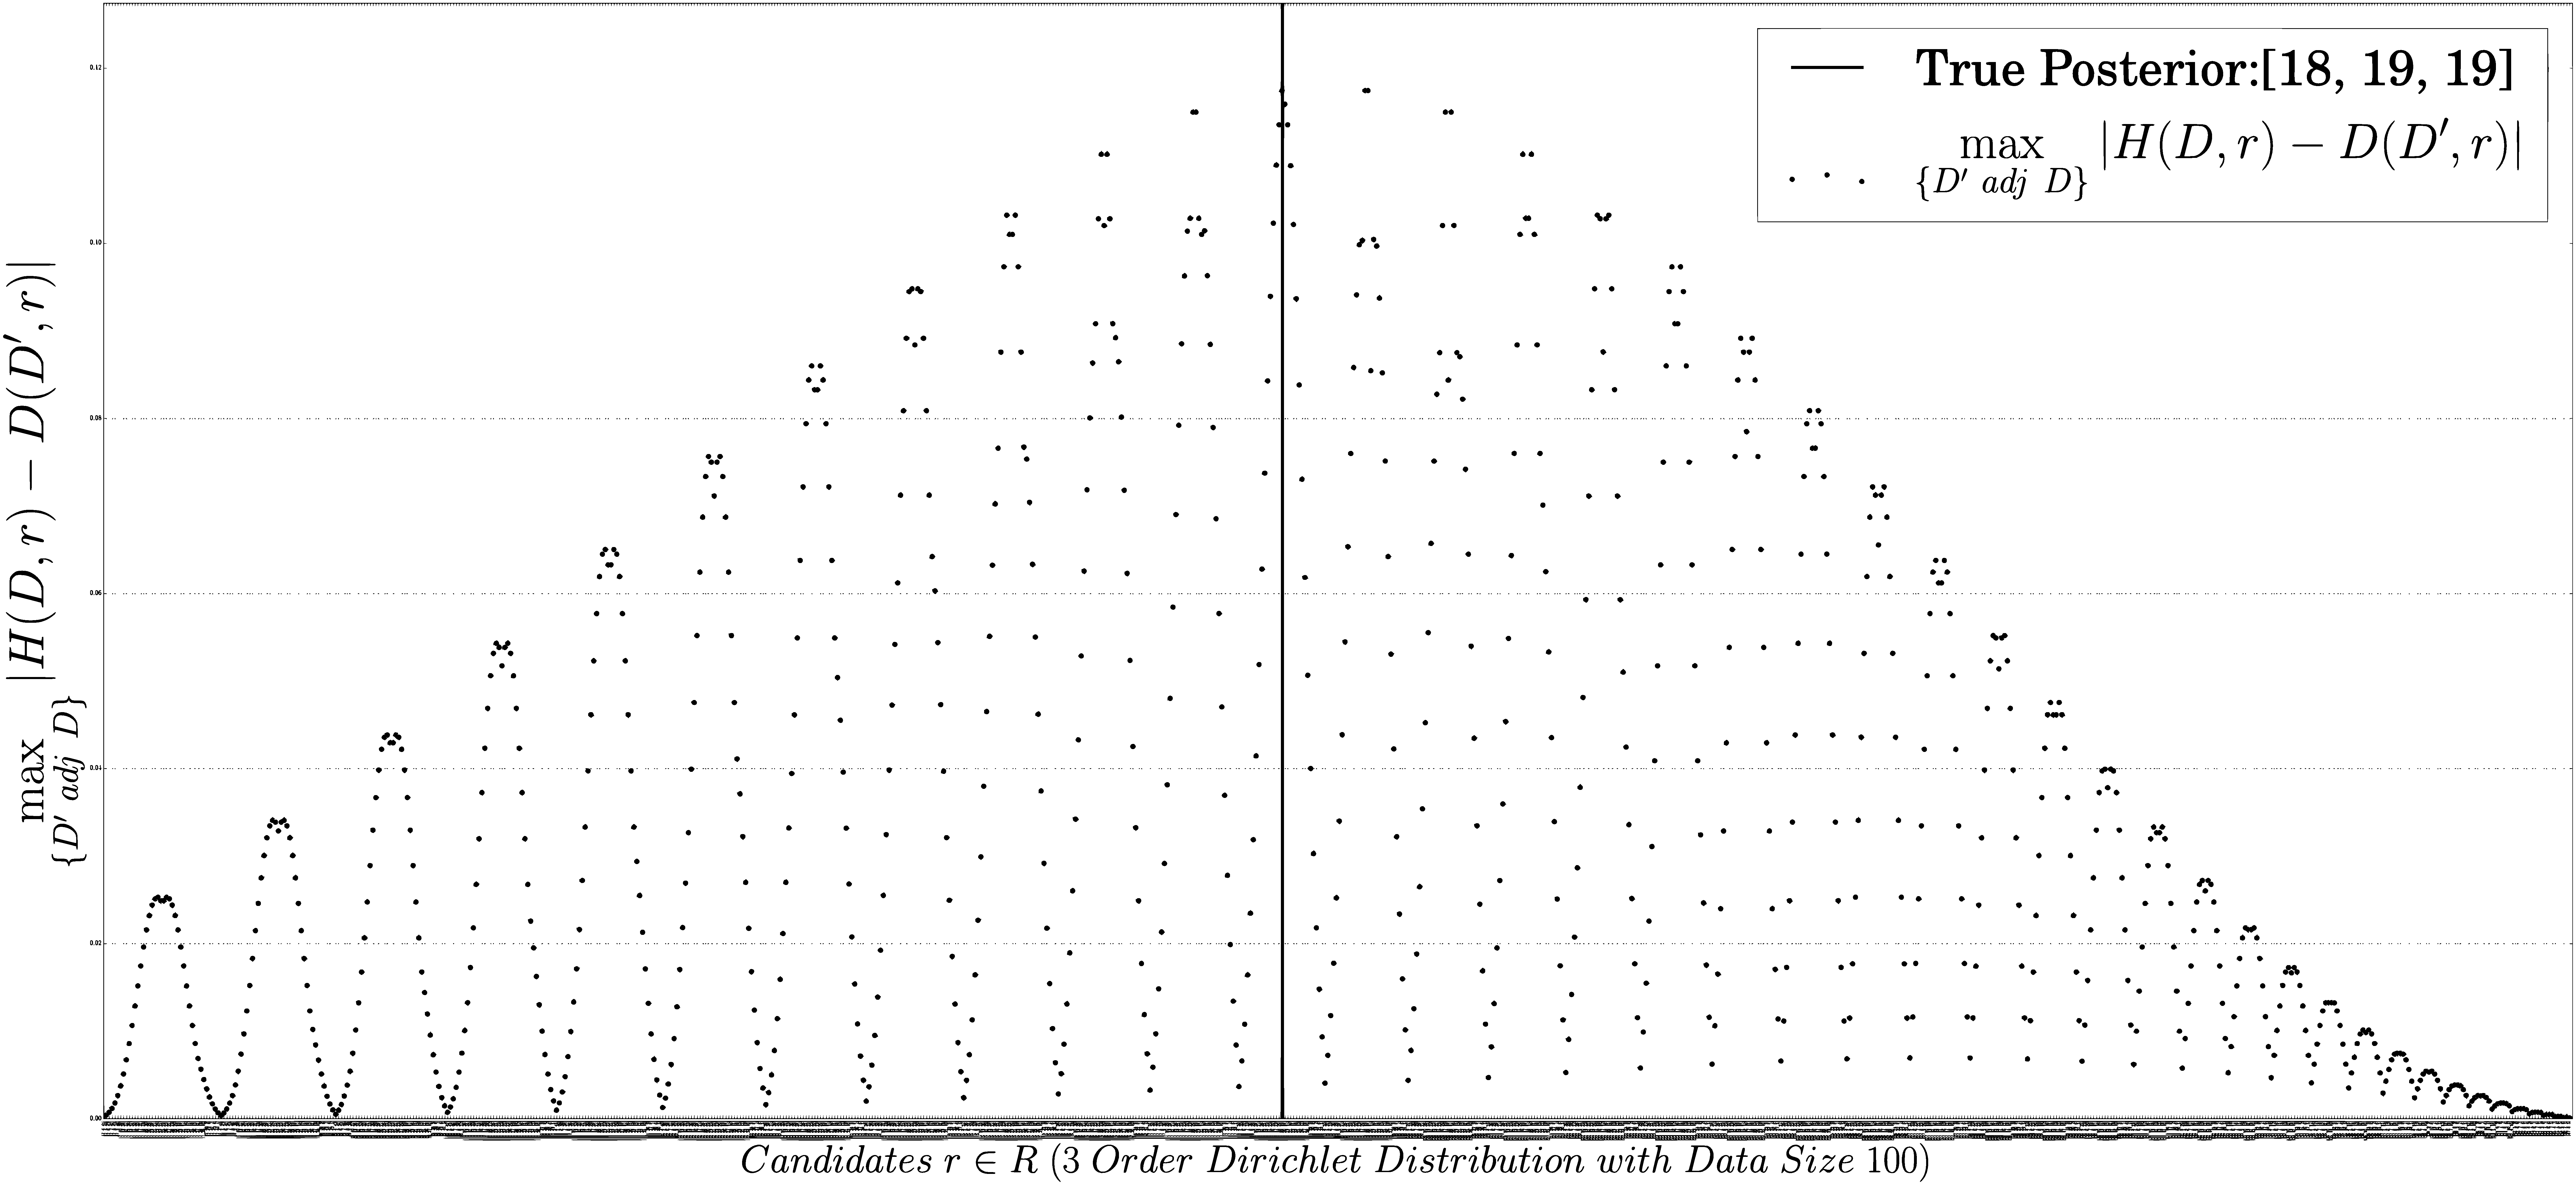
\includegraphics[width=0.45\textwidth]{efficiency.eps}
\caption{Experimental Results for Finding the Local Sensitivity Efficiently}
\label{fig_efficiency}
\end{figure}

\subsection{Accuracy Evaluation}
\subsubsection{Theoretical Results}
In Fig. \ref{fig_theory} and \ref{fig_theory_epsilon}, we plot on the x-axis the Hellinger distance from the true posterior and on the y-axis the theoretical probabilities of outputting the candidates with that distance under the different mechanisms. We consider \emph{balanced} data sets, which means that in the Beta-Binomial model (Figure \ref{subfig_theory_2d}) the datasets will consist of 50\% 1s and the rest 0s, while for the
Dirichelet-Multinomial (Figure  \ref{subfig_theory_3d})
the data will be split in the $k=3$ bins with perecentages of: 33\%, 33\% and 34\% in 3 dimensionality. Same concept in 4 dimensionality.

We consider 5 mechanisms in our comparison experiments, including the Laplace mechanism ($\lapmech$), improved Laplace mechanism ($\ilapmech$), standard exponential mechanism ($\mathsf{expMech}$), non-private exponential mechanism ($\lexpmech$) and the newly designed mechanisms ($\hexpmech$ with $\gamma$ sensitivity achieving $\epsilon-$dp).

\begin{figure}
\begin{center}
\centering
  \subfigure[2 dimensions, data size $600$]{
    \includegraphics[width=0.22\textwidth]{theory_2d.eps}
  \label{subfig_theory_2d}
  }
  \subfigure[3 dimensions, data size $600$]{
    \includegraphics[width=0.22\textwidth]{theory_3d.eps}
  \label{subfig_theory_3d}
  }
\caption{The theory probabilities of outputting candidates in certain distance from true posterior, with balanced data set and parameters $\epsilon = 1.0$}
\label{fig_theory}
\end{center}
\end{figure}

Candidates of smaller distance from true posterior are considered to be good results, which can result in good accuracy. From Fig. \ref{fig_theory}, it can be derived that all these mechanisms (except standard exponential mechanism $\expmech$ in green line) can output good results with larger probability. The $\lexpmech$ can output good results with higher probability than others, but $\lexpmech$ is non-private. For these are $\epsilon -$differentially private, the improved laplace mechanism $\ilapmech$ with $\ell_1$ norm metric can produce good results with higher probability, i.e., perform better in terms of accuracy than others. As the dimension increases from 2 to 3, mechanisms' behavior remain the same.

\begin{figure}
\begin{center}
\centering
  \subfigure[data size 1000]{
    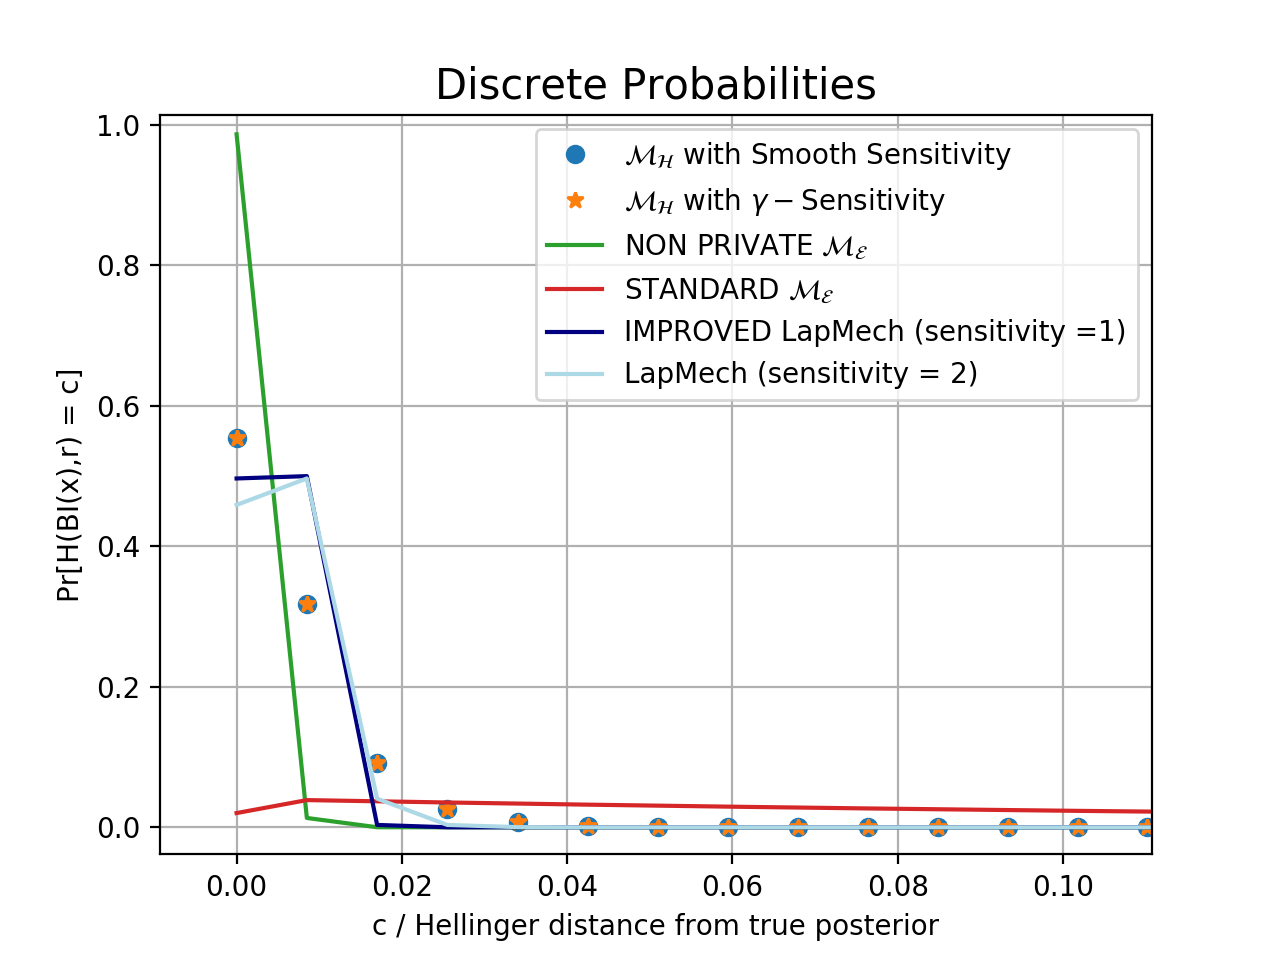
\includegraphics[width=0.22\textwidth]{epsilon5_2d_1000.eps}
  \label{subfig_theory_2d}
  }
  \subfigure[data size 10000]{
    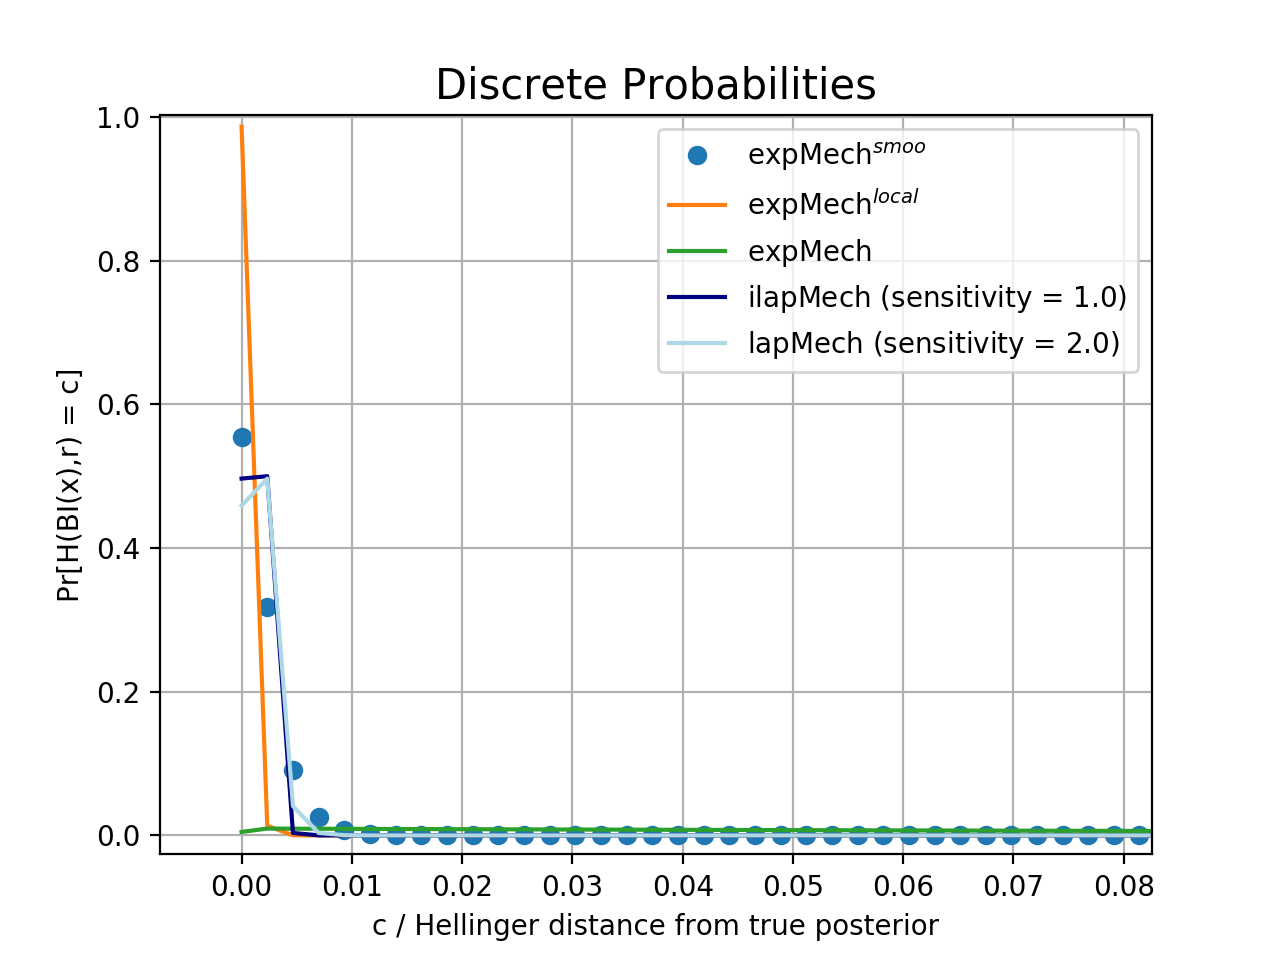
\includegraphics[width=0.22\textwidth]{epsilon5_2d_10000.eps}
  \label{subfig_theory_3d}
  }
\caption{The theory probabilities of outputting candidates in certain distance from true posterior, with balanced data set and parameters $\epsilon = 5.0$, in 2 dimensions}
\label{fig_theory_epsilon}
\end{center}
\end{figure}

Increasing the privacy bound $\epsilon$, we get theoretical results as in Fig. \ref{fig_theory_epsilon} in 2 dimensions. The $\lexpmech$ is still the one with the best accuracy, but it is non-private. However, the $\lapmech$ and $\ilapmech$ having the similar performance, and $\hexpmech$ can produce the correct posterior with higher probability than the others. And the standard exponential mechanism $\expmech$ is still the worst one.


\subsubsection{Experimental Results}
\label{subsec_vs_variables}

In this section, we evaluate the accuracy of the mechanisms defined in
Section (\ref{sec_mechs}) w.r.t. four variables, including data size, dimensions,
data variance, prior distribution, and some combinations thereof.
Every plot is an average over 1000 runs. In all the experiments we set
$\epsilon = 1.0$.

\noindent In the following some of the plots show
mean error as a function of the datasize while one
is a whiskers-plot where the y-axis shows the average
accuracy (or equivalently, the error) of the mechanisms, and the x-axis, instead shows
different balanced priors used. The boxes extend from the lower to the upper quartile values
of the data, with a line at the median. A notch on the box around the
median is also drawn to give a rough guide to the significance of
difference of medians; The whiskers extend from the box to show the
range of the data. A blue box in the plots represents the $\hexpmech$'s behavior-- where the sensitivity is calibrated
w.r.t Hellinger distance-- while the green box next to
it represents the performance of a variation of the basic Laplace
mechanism $\lapmech$, and red one is $\ilapmech$ presented in Section (\ref{sec_mechs}) with the same
settings: that is $\epsilon$, data, prior. The variation
considered performs a postprocessing on the released parameters so
that they are consistent. For instance when the sum of the noised
parameters is greater than $n$ we will truncate them so that they sum
up to $n$.

\paragraph{Increasing data size with balanced datasets}
\label{subsubsec_vs_datasize}


\begin{figure}[ht]
\begin{center}
\centering
\subfigure[Increasing data size with prior $\betad(1,1)$, balanced datasets and parameters $\epsilon = 1.0$]
{ \includegraphics[width=0.35\textwidth]{sampling_2d.eps}
\label{fig_vs_datasize_2d}
}

\subfigure[Increasing data size with $\dirichlet(1,1,1)$ prior distribution, balanced datasets and parameters $\epsilon = 1.0$]
{
  \includegraphics[width=0.35\textwidth]{sampling_3d.eps} 
  \label{fig_vs_datasize_3d}
}
\subfigure[Increasing data size with $\dirichlet(1,1,1,1)$ prior distribution, balanced datasets and parameters $\epsilon = 1.0$]
{
  \includegraphics[width=0.35\textwidth]{sampling_4d.eps} 
  \label{fig_vs_datasize_4d}
}
\end{center}
\end{figure}

In Figures \ref{fig_vs_datasize_2d}, \ref{fig_vs_datasize_3d} and \ref{fig_vs_datasize_4d} we still consider \emph{balanced} data sets
of observations. The results show that when the data size increases, the average errors of
$\hexpmech$, $\lapmech$ and $\ilapmech$ decrease. For small datasets,
i.e with size less $300$ in the case of Beta-Binomial models, the Laplace mechanisms outperform $\hexpmech$.
But for bigger data sets, that is, bigger than $300$, or as in Figure \ref{fig_vs_datasize_2d} where
we considered data sets of the order of 15 thousands elements,
the $\hexpmech$ outperforms the $\lapmech$, and asymptotically approaches the improved Laplace mechanism $\ilapmech$.
Similar experimental tendencies were obtained for the Dirichlet-multinomial model (Figure \ref{fig_vs_datasize_3d} and \ref{fig_vs_datasize_4d}).


\paragraph{Fixed dataset varying balanced priors}
\label{subsubsec_vs_prior}
In Figure \ref{fig_vs_prior}, we fix the data set to be $(50,50)$, and the parameters the same as before: $\epsilon = 1.0$ and $\delta = 10^{-8}$ . We studied the accuracy under different priors, where the priors considered  are also balanced.
Similar to the plots above, Figure \ref{fig_vs_prior} shows that in the beginning the baseline Laplace mechanism and improved Laplace mechanism performs better but the baseline approach is outperformed after a while, and very close to the improved Laplace mechanism.
\begin{figure}
\centering
\includegraphics[width=0.35\textwidth]{sampling_prior.eps}
\caption{Observed data set is: $(50,50)$, varying balanced priors}
\label{fig_vs_prior}
\end{figure}

\subsection{Privacy Evaluation}
\label{subsec_experiment_privacy}
In order to see our privacy behavior, we study the accurate epsilon under concrete cases in this section. The $(\epsilon, \delta)$ - differential privacy we proved in Sec. \ref{subsec_hexpmech} is just an upper bound, we concrete $\epsilon$ should be smaller than upper bound in our exponential mechanism. We calculate the concrete privacy value in following ways wrt. the data size, and obtain plots in Fig. \ref{fig_privacy}.

\begin{figure}
\begin{center}
\centering
    \includegraphics[width=0.35\textwidth]{privacyloss.eps}
\caption{Actual privacy loss of different data size when privacy bound $\epsilon = 1.0$ in 2 dimensions, prior:$\betad(1,1)$ and balanced data}
\label{fig_privacy}
\end{center}
\end{figure}

$\epsilon = 1.0$ is a privacy upper bound, we can observe that the concrete $\epsilon$ values are smaller than the upper bound. That is to say, we achieved a higher privacy level than expected. 



\section{Related Work}

A plentiful of data analysis algorithms have been studied to preserve differential privacy, including the subspace clustering algorithm \cite{wang2015differentially}, the gradient decedent algorithm in deep learning \cite{abadi2016deep}, logical regression \cite{chaudhuri2009privacy}, principle component analysis \cite{chaudhuri2012near}, probabilitic inference \cite{williams2010probabilistic} and convergence in statistic estimation \cite{chaudhuri2012convergence}, etc. 

In Bayesian Inference data analysis, mechanisms are proposed corresponded to maintain their differential privacy, focusing on 3 different goals: 1) Inherited differential privacy property of posterior sampling in Bayesian inference. \cite{dimitrakakis2014robust}, \cite{zhang2016differential}, \cite{zheng2015differential} and \cite{wang2015privacy}. 2) Data sampled and released from posterior distribution of Bayesian is differentially private \cite{Zhang2017privbayes}, \cite{dimitrakakis2015differential},  \cite{foulds2016theory}. 3) The inference process is differentially private and the posterior distribution released should be private itself, in the meantime, with good accuracy. The third topic where our work focus on is still very new. moreover, their design spaces are more specific to the $\ell_1$ norm and Laplace mechanism. That's why we explore different metrics and different algorithms over the design space.


\section{Conclusion}
From what we have seen in the previous sections we can obtain following conclusions. We explored the design space of the mechanisms for differentially privacy Bayesian inference, by considering different metrics and different algorithms.
\begin{itemize}
  \item The accuracy can change a lot when considering different metrics and using different sensitivity values.
  \item Different algorithms have different performance w.r.t. different aspect. From the experimental results, Laplace mechanism family have a good efficiency and accuracy when using $\ell_1$ norm metric. But exponential mechanism family can be a good application when considering different metrics.
\end{itemize}


\bibliography{bysinfer}
\bibliographystyle{icml2019}

\newpage
\section*{Appendix I}
\label{app_sensitivity}
\begin{proof}
of Theorem. \ref{thm_gamma_smooth}.\\
For $\adj{\dataobs}{\dataobs'}$ and arbitrary $\dataobs'' \in \{0,1\}^{n}$:\\
From Equation (\ref{eq_smooth}), we can get:
\[
\frac{1}{S(\dataobs)} 
 = \min_{\dataobs'' \in \{0,1\}^{n}}\bigg \{ \frac{1}{LS(\dataobs'')} +\gamma \cdot d(\dataobs,\dataobs'') \bigg \}\\
\]

Since $d(\dataobs,\dataobs'') \leq d(\dataobs,\dataobs') + d(\dataobs',\dataobs'') \leq 1 + d(\dataobs',\dataobs'')$:

\begin{equation*}
\begin{split}
& \leq \min_{\dataobs'' \in \{0,1\}^{n}}\bigg \{  \frac{1}{LS(\dataobs'')} +\gamma \cdot (1 + d(\dataobs',\dataobs'')) \bigg \}\\
& = \min_{\dataobs'' \in \{0,1\}^{n}}\bigg \{
\gamma + \frac{1}{LS(\dataobs'')} +\gamma \cdot d(\dataobs',\dataobs'')\bigg 
\}\\
& = \gamma + \min_{\dataobs'' \in \{0,1\}^{n}}\bigg \{
\frac{1}{LS(\dataobs'')} +\gamma \cdot d(\dataobs',\dataobs'')\bigg
\}\\
& = \gamma + \frac{1}{S(\dataobs')}
\end{split}
\end{equation*}
Then we can get:
$\frac{1}{S(\dataobs)} - \frac{1}{S(\dataobs')} \leq \gamma.$
\end{proof}

\section*{Appendix II}
\label{app_privacyproof}
\begin{proof} of Lemma \ref{lem_hexpmech_privacy}.\\
  By Definition \ref{def_epsilon_dp}, to proof Lemma \ref{lem_hexpmech_privacy}, we need to prove:\\
  For any $\adj{\dataobs}{\dataobs'} \in \mathcal{X}$ and any beta distribution $r$:
  \begin{equation*}
  \hexpmechPr{\dataobs}{z = r} \leq e^{\epsilon} \hexpmechPr{\dataobs'}{z = r}. 
  \end{equation*}
  By definition \ref{def_smoo_2}:
  \begin{equation*}
  \begin{split}
  \hexpmechPr{\dataobs}{z = r} 
  & = \frac {\exp\big(\frac{-\epsilon\cdot\ux{r}}{4\cdot S(\dataobs)}\big)}{\unomalizer{\dataobs}} \\
  & = \frac {\exp\big(
  \frac{-\epsilon\cdot(\ux{r} + \uxadj{r} - \uxadj{r})}{4\cdot S(\dataobs)}
  \big)}
  {\unomalizer{\dataobs}} \\
  & = \frac {\exp\big(
  \frac{-\epsilon\cdot(\uxadj{r})}{4\cdot S(\dataobs)}
  \big)}
  {\unomalizer{\dataobs}}
  \\
  & \cdot \exp\big( \frac{\epsilon\cdot(\uxadj{r} - \ux{r})}{4\cdot S(\dataobs)} \big)\\
  \end{split}
  \end{equation*}
  Because $S(\dataobs) \geq LS(\dataobs) \geq (\uxadj{r} - \ux{r})$:
  \begin{equation*}
  \begin{split}
  & \leq \frac {exp\big(
  \frac{-\epsilon\cdot(\uxadj{r})}{4\cdot S(\dataobs)}
  \big)}
  {\unomalizer{\dataobs}}
  \cdot \exp\big( \frac{\epsilon}{4} \big) \\
  & = \exp\big( \frac{\epsilon}{4} \big) \cdot 
  \frac {
  \exp
  \big(
  \frac{-\epsilon\cdot(\uxadj{r})}{4\cdot S(\dataobs)}
  \big)
  } 
  {\unomalizer{\dataobs}}\\
  & \cdot \exp
  \big(
  \frac{\epsilon\cdot(\uxadj{r})}{4\cdot S(\dataobs')}
  \big)
  \exp
  \big(
  \frac{-\epsilon\cdot(\uxadj{r})}{4\cdot S(\dataobs')}
  \big)\\
  & = \exp\big( \frac{\epsilon}{4} \big) \cdot 
  \frac {
  \exp
  \big(
  \frac{-\epsilon\cdot(\uxadj{r})}{4\cdot S(\dataobs')}
  \big)
  } 
  {\unomalizer{\dataobs}}\\
  & \cdot \exp
  \big(
  \frac{\epsilon\cdot(\uxadj{r})}{4}(\frac{1}{S(\dataobs')} - \frac{1}{S(\dataobs)})
  \big)\\
  \end{split}
  \end{equation*}
  
  Because $\uxadj{r} = \hellinger(\bysinfer(\dataobs'), r) \leq 1$:
  \begin{equation*}
  \begin{split}
  & \leq \exp\big( \frac{\epsilon}{4} \big) \cdot 
  \frac {
  \exp
  \big(
  \frac{-\epsilon\cdot(\uxadj{r})}{4\cdot S(\dataobs')}
  \big)
  } 
  {\unomalizer{\dataobs}}\\
  & \cdot \exp
  \big(
  \frac{\epsilon}{4}(\frac{1}{S(\dataobs')} - \frac{1}{S(\dataobs)})
  \big)\\
  \end{split}
  \end{equation*}

  Because the property of $\gamma -$smooth sensitivity: $\frac{1}{S(\dataobs')} - \frac{1}{S(\dataobs)} \leq \gamma$:  
  \begin{equation*}
  \begin{split}
  & \leq \exp\big( \frac{\epsilon}{4} \big) \cdot 
  \frac {
  \exp
  \big(
  \frac{-\epsilon\cdot(\uxadj{r})}{4\cdot S(\dataobs')}
  \big)
  } 
  {\unomalizer{\dataobs}}
  \exp
  \big(
  \frac{\epsilon}{4} \cdot \gamma
  \big)\\
  & = \exp\big( \frac{\epsilon}{4} + \frac{\epsilon}{4} \cdot \gamma\big) \cdot 
  \frac {
  \exp
  \big(
  \frac{-\epsilon\cdot(\uxadj{r})}{4\cdot S(\dataobs')}
  \big)
  } 
  {\unomalizer{\dataobs}}\\
  \end{split}
  \end{equation*}

  Doing the same transformation in the denominator:
  \begin{equation*}
  \begin{split}
  & = \exp\big( \frac{\epsilon}{4} + \frac{\epsilon}{4} \cdot \gamma\big) \cdot 
  \frac {
  \exp
  \big(
  \frac{-\epsilon\cdot(\uxadj{r})}{4\cdot S(\dataobs')}
  \big)
  } 
  {
  \sum_{r'\in \candidateset} 
  \exp 
  \big(
  \frac{-\epsilon\cdot(\ux{r'} + \uxadj{r'} - \uxadj{r'})}{4 \cdot S(\dataobs)}
  \big)
  }\\
  & = \exp\big( \frac{\epsilon}{4} + \frac{\epsilon}{4} \cdot \gamma\big) \\
  & \cdot 
  \frac {
  \exp
  \big(
  \frac{-\epsilon\cdot(\uxadj{r})}{4\cdot S(\dataobs')}
  \big)
  } 
  {
  \sum_{r'\in \candidateset} 
  \exp 
  \big(
  \frac{-\epsilon\cdot(\uxadj{r'}}{4 \cdot S(\dataobs)}
  \big)
  \exp 
  \big(
  \frac{-\epsilon\cdot(\ux{r'} - \uxadj{r'})}{4 \cdot S(\dataobs)}
  \big)
  }\\
  \end{split}
  \end{equation*}

  Because $S(\dataobs) \geq LS(\dataobs) \geq (\ux{r} - \uxadj{r})$ $\implies$ $ \frac{-\epsilon\cdot(\ux{r'} - \uxadj{r'})}{4 \cdot S(\dataobs)} \geq \frac{-\epsilon}{4}$:
  \begin{equation*}
  \begin{split}
  & \leq \exp\big( \frac{\epsilon}{4} + \frac{\epsilon}{4} \cdot \gamma\big) \cdot 
  \frac {
  \exp
  \big(
  \frac{-\epsilon\cdot(\uxadj{r})}{4\cdot S(\dataobs')}
  \big)
  } 
  {
  \sum_{r'\in \candidateset} 
  \exp 
  \big(
  \frac{-\epsilon\cdot(\uxadj{r'}}{4 \cdot S(\dataobs)}
  \big)
  \exp 
  \big(
  \frac{-\epsilon}{4}
  \big)
  }\\
  & = \exp\big( \frac{\epsilon}{4} + \frac{\epsilon}{4} \cdot \gamma\big) \cdot 
  \frac {
  \exp
  \big(
  \frac{-\epsilon\cdot(\uxadj{r})}{4\cdot S(\dataobs')}
  \big)
  } 
  {
  \sum_{r'\in \candidateset} 
  \exp 
  \big(
  \frac{-\epsilon\cdot(\uxadj{r'}}{4 \cdot S(\dataobs)}
  \big)
  }\\
  & \cdot 
  \frac{1}
  {
  \exp 
  \big(
  \frac{-\epsilon}{4}
  \big)
  \exp
  \big(
  \frac{\epsilon\cdot(\uxadj{r'})}{4\cdot S(\dataobs')}
  \big)
  \exp
  \big(
  \frac{-\epsilon\cdot(\uxadj{r'})}{4\cdot S(\dataobs')}
  \big)
  }\\
  & = \exp\big( \frac{\epsilon}{4} + \frac{\epsilon}{4} \cdot \gamma\big) \cdot 
  \frac {
  \exp
  \big(
  \frac{-\epsilon\cdot(\uxadj{r})}{4\cdot S(\dataobs')}
  \big)
  } 
  {
  \sum_{r'\in \candidateset} 
  \exp 
  \big(
  \frac{-\epsilon\cdot(\uxadj{r'}}{4 \cdot S(\dataobs')}
  \big)}\\
  & \cdot\frac{1}{
  \exp 
  \big(
  \frac{-\epsilon}{4}
  \big)
  \exp
  \big(
  \frac{- \epsilon\cdot(\ux{r'})}{4}
  (\frac{1}{S(\dataobs)}
-
  \frac{1}{S(\dataobs')})
  \big)
  }
  \end{split}
  \end{equation*}

  Because $\uxadj{r} = \hellinger(\bysinfer(\dataobs'), r) \leq 1$ $\implies$ $\frac{- \epsilon\cdot(\ux{r'})}{4} \geq  \frac{-\epsilon}{4}$:
  \begin{equation*}
  \begin{split}
  & \leq \exp\big( \frac{\epsilon}{4} + \frac{\epsilon}{4} \cdot \gamma\big) \cdot 
  \frac {
  \exp
  \big(
  \frac{-\epsilon\cdot(\uxadj{r})}{4\cdot S(\dataobs')}
  \big)
  } 
  {
  \sum_{r'\in \candidateset} 
  \exp 
  \big(
  \frac{-\epsilon\cdot(\uxadj{r'}}{4 \cdot S(\dataobs')}
  \big)}\\
  & \cdot \frac{1}{
  \exp 
  \big(
  \frac{-\epsilon}{4}
  \big)
  \exp
  \big(
  \frac{- \epsilon}{4}
  (\frac{1}{S(\dataobs)}
-
  \frac{1}{S(\dataobs')})
  \big)
  }\\
  \end{split}
  \end{equation*}

  Because the property of $\gamma -$ smooth sensitivity: $\frac{1}{S(\dataobs)} - \frac{1}{S(\dataobs')} \leq \gamma$ $\implies$
  $\frac{- \epsilon}{4}
  (\frac{1}{S(\dataobs)}-
  \frac{1}{S(\dataobs')}) \geq \frac{- \epsilon}{4} \cdot \gamma$
  \begin{equation*}
  \begin{split}
  & \leq \exp\big( \frac{\epsilon}{4} + \frac{\epsilon}{4} \cdot \gamma\big) \cdot 
  \frac {
  \exp
  \big(
  \frac{-\epsilon\cdot(\uxadj{r})}{4\cdot S(\dataobs')}
  \big)
  } 
  {
  \sum_{r'\in \candidateset} 
  \exp 
  \big(
  \frac{-\epsilon\cdot(\uxadj{r'}}{4 \cdot S(\dataobs')}
  \big)
  \exp 
  \big(
  \frac{-\epsilon}{4}
  \big)
  \exp
  \big(
  \frac{- \epsilon}{4} \cdot \gamma
  \big)
  }\\
  & = \exp\big( \frac{\epsilon}{4} + \frac{\epsilon}{4} \cdot \gamma\big) \cdot 
  \frac {
  \exp
  \big(
  \frac{-\epsilon\cdot(\uxadj{r})}{4\cdot S(\dataobs')}
  \big)
  } 
  {
  \sum_{r'\in \candidateset} 
  \exp 
  \big(
  \frac{-\epsilon\cdot(\uxadj{r'}}{4 \cdot S(\dataobs')}
  \big)
  \exp 
  \big(
  \frac{-\epsilon}{4} +   \frac{- \epsilon}{4} \cdot \gamma
  \big)
  }\\
  & = e^{( \frac{\epsilon}{2} + \frac{\epsilon}{2} \cdot \gamma )} \cdot 
  \frac {
  \exp
  \big(
  \frac{-\epsilon\cdot(\uxadj{r})}{4\cdot S(\dataobs')}
  \big)
  } 
  {
  \unomalizer{\dataobs'}
  }\\
  & = e^{( \frac{\epsilon}{2} + \frac{\epsilon}{2} \cdot \gamma )} \cdot   \hexpmechPr{\dataobs'}{z = r}
  \end{split}
  \end{equation*}

  Given $\gamma = 1$, $\epsilon - $differential privacy can be achieved by $\hexpmech$.


\end{proof}
\end{document}

